\documentclass[12pt,addpoints]{repaso}
\grado{2}
\nivel{Secundaria}
\cicloescolar{2024-2025}
\materia{Ciencias y Tecnología: Física \normalfont \color{darkgray}  \small con adecuación curricular.}
\unidad{2}
\title{Practica la Unidad}
\aprendizajes{
\item Identifica problemas de la vida cotidiana y plantea soluciones.\\[-1.2em]
\item Conoce y caracteriza el pensamiento científico para plantearse y resolver problemas en la escuela y su cotidianidad.\\[-1.2em]
\item Identifica cuáles son, cómo se definen y cuál es la simbología de las unidades básicas y derivadas del Sistema Internacional de Unidades.\\[-1.2em]
\item Relaciona e interpreta las teorías sobre estructura de la materia, a partir de los modelos atómicos y de partículas y los fenómenos que les dieron origen.\\[-1.2em]
\item Interpreta la temperatura y el equilibrio térmico con base en el modelo de partículas.\\[-1.2em]
}
\author{Melchor Pinto, J.C.}
\begin{document}%\vfill
\INFO%\afterpage{\blankpage}%
% \begin{multicols}{2}
%\tableofcontents
% \end{multicols}
%\newpage

\begin{questions}%\large

	% \addcontentsline{toc}{section}{Unidad 2}
	% \section*{Unidad 2}

	\questionboxed[12]{Elige la respuesta correcta.

	\begin{multicols}{2}
		\begin{parts}
			\part Es el espacio que ocupa un objeto.

			\begin{choices}
				\choice Masa  \choice Densidad  \CorrectChoice Volumen  \choice Materia
			\end{choices}

			\part ¿Qué es la materia?

			\begin{choices}
				\choice La capacidad que tiene un objeto para interactuar con otros \choice El producto de la aceleración por la masa \choice Todo lo que ocupa un lugar en el espacio \choice Todo lo que se puede detectar
			\end{choices}

			\part Es la cantidad de materia que posee un cuerpo.

			\begin{choices}
				\CorrectChoice Masa  \choice Densidad  \choice Volumen  \choice Materia
			\end{choices}

			\part  Es todo aquello que ocupa un lugar en espacio.

			\begin{choices}
				\choice Masa  \choice Densidad  \choice Volumen  \CorrectChoice Materia
			\end{choices}

			\part La materia \dots

			\begin{choices}
				\choice no se puede medir.  \choice es detectable con distintos medios.  \choice no se puede observar.  \choice no ocupa un lugar en el espacio.
			\end{choices}

			\part Son propiedades de la materia:

			\begin{choices}
				\choice aceleración y fuerza.  \choice distintos medios de propagación.  \choice emoción y sueño.  \choice forma, volumen, masa y compresibilidad.
			\end{choices}
		\end{parts}
	\end{multicols}
	}

	\questionboxed[10]{Señala si son verdaderas o falsas las siguientes afirmaciones:

		\begin{multicols}{2}
			\begin{parts}
				\part La velocidad y la rapidez se miden en unidades distintas.

				\begin{oneparcheckboxes}
					\choice Verdadero \CorrectChoice Falso
				\end{oneparcheckboxes}

				\part No es lo mismo desplazamiento que trayectoria.

				\begin{oneparcheckboxes}
					\CorrectChoice Verdadero \choice Falso
				\end{oneparcheckboxes}

				\part La rapidez tiene magnitud y direcci\'on.

				\begin{oneparcheckboxes}
					\choice Verdadero \CorrectChoice Falso
				\end{oneparcheckboxes}

				\part La rapidez es el cociente de la distancia recorrida por un objeto y el tiempo que tarda en recorrerla.

				\begin{oneparcheckboxes}
					\CorrectChoice Verdadero \choice Falso
				\end{oneparcheckboxes}

				\part La rapidez es el movimiento a gran velocidad.

				\begin{oneparcheckboxes}
					\choice Verdadero \CorrectChoice Falso
				\end{oneparcheckboxes}

				\part La distancia siempre es una cantidad positiva.

				\begin{oneparcheckboxes}
					\CorrectChoice Verdadero \choice Falso
				\end{oneparcheckboxes}

				\part En la aceleración se recorren distancias iguales en tiempos iguales.

				\begin{oneparcheckboxes}
					\choice Verdadero \CorrectChoice Falso
				\end{oneparcheckboxes}

				\part La aceleración es el cambio en el valor de la velocidad.

				\begin{oneparcheckboxes}
					\choice Verdadero \CorrectChoice Falso
				\end{oneparcheckboxes}

				\part La aceleración es una variable cinemática.

				\begin{oneparcheckboxes}
					\CorrectChoice Verdadero \choice Falso
				\end{oneparcheckboxes}

				\part La aceleración se mide en las mismas unidades que la velocidad.

				\begin{oneparcheckboxes}
					\choice Verdadero \CorrectChoice Falso
				\end{oneparcheckboxes}
			\end{parts}
		\end{multicols}
	}

	

	\questionboxed[8]{\include*{../questions/question034}}

	\questionboxed[18]{Coloca los conceptos en el lugar que les corresponda en la imagen.\\

		\begin{minipage}[t][][b]{.2\textwidth}
			\wordpill{Modelo atómico del ``panqué con pasas''}
			\wordpill{El descubrimiento del núcleo atómico}
			\wordpill{El descubrimiento del electrón}
			\wordpill{Ernest Rutherford}
			\wordpill{Neutrones}
			\wordpill{Niels Bohr}
			\wordpill{Modelo Cuántico del átomo}
			\wordpill{Explicar los espectros luminosos}
			\wordpill{Descubrir el átomo de hidrógeno}
		\end{minipage}\qquad\quad\hfill%
		\begin{minipage}[t][][b]{.7\textwidth}
			\ifprintanswers{
				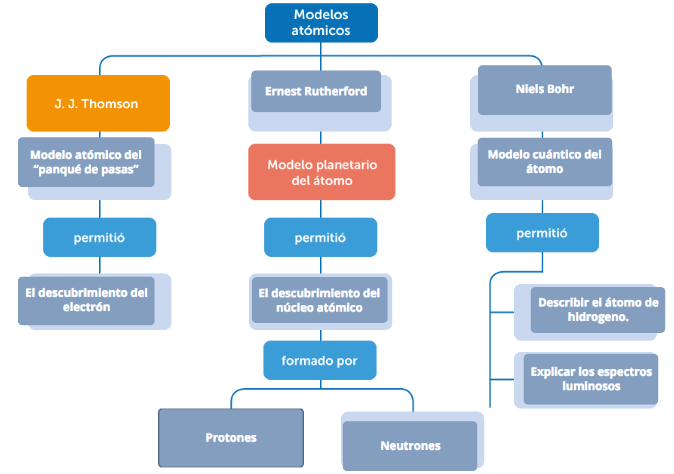
\includegraphics[width=\textwidth]{../images/SINFI_U2_AC65_IMGS1_sol.png}
			}\else{
				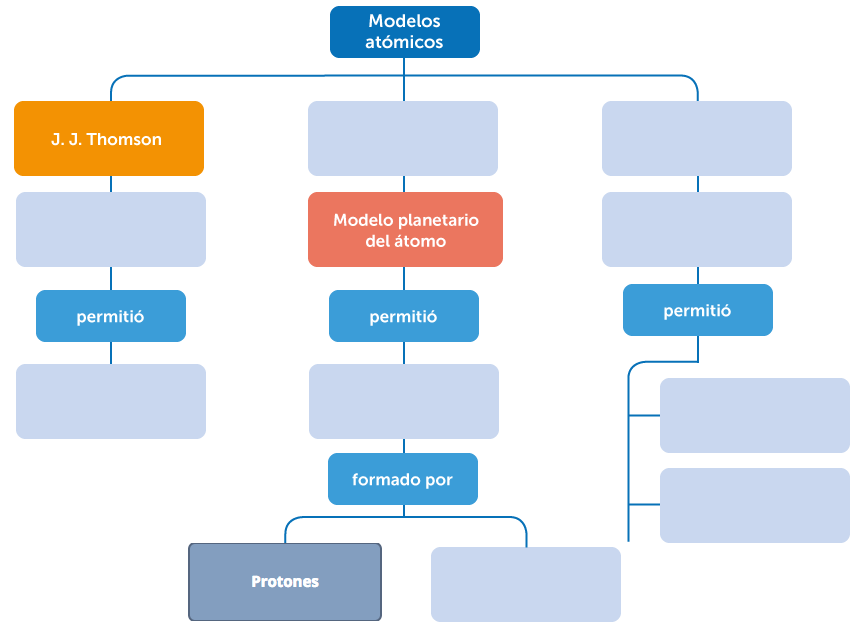
\includegraphics[width=\textwidth]{../images/SINFI_U2_AC65_IMGS1.png}
			}\fi         
		 \end{minipage}
	}

	\questionboxed[10]{Señala si son verdaderas o falsas las siguientes afirmaciones:
	\begin{multicols}{2}
		\begin{parts}
			\part La velocidad y la rapidez se miden en unidades distintas.

			\begin{oneparcheckboxes}
				\choice Verdadero \CorrectChoice Falso
			\end{oneparcheckboxes}
			\part No es lo mismo desplazamiento que trayectoria.

			\begin{oneparcheckboxes}
				\CorrectChoice Verdadero \choice Falso
			\end{oneparcheckboxes}
			\part La rapidez tiene magnitud y direcci\'on.

			\begin{oneparcheckboxes}
				\choice Verdadero \CorrectChoice Falso
			\end{oneparcheckboxes}
			\part La rapidez es el cociente de la distancia recorrida por un objeto y el tiempo que tarda en recorrerla.

			\begin{oneparcheckboxes}
				\CorrectChoice Verdadero \choice Falso
			\end{oneparcheckboxes}
			\part La rapidez es el movimiento a gran velocidad.

			\begin{oneparcheckboxes}
				\choice Verdadero \CorrectChoice Falso
			\end{oneparcheckboxes}
			\part La distancia siempre es una cantidad positiva.

			\begin{oneparcheckboxes}
				\CorrectChoice Verdadero \choice Falso
			\end{oneparcheckboxes}
			\part En la aceleración se recorren distancias iguales en tiempos iguales.

			\begin{oneparcheckboxes}
				\choice Verdadero \CorrectChoice Falso
			\end{oneparcheckboxes}
			\part La aceleración es el cambio en el valor de la velocidad.

			\begin{oneparcheckboxes}
				\choice Verdadero \CorrectChoice Falso
			\end{oneparcheckboxes}
			\part La aceleración es una variable cinemática.

			\begin{oneparcheckboxes}
				\CorrectChoice Verdadero \choice Falso
			\end{oneparcheckboxes}
			\part La aceleración se mide en las mismas unidades que la velocidad.

			\begin{oneparcheckboxes}
				\choice Verdadero \CorrectChoice Falso
			\end{oneparcheckboxes}
		\end{parts}
	\end{multicols}
}

	\questionboxed[9]{Señala si son \textit{verdaderas} o \textit{falsas} las siguientes frases:

		\begin{multicols}{2}
			\begin{parts}
				\part Los electrones son partículas tan pequeñas que no es posible observarlas a simple vista, pero podemos saber de ellas a través de fenómenos como la electricidad, los espectros luminosos y el magnetismo.

				\begin{oneparchoices}
					\CorrectChoice Verdadero \choice Falso
				\end{oneparchoices}

				\part Los electrones son partículas de carga negativa cubiertas por una nube de carga positiva; la magnitud de ambas cargas es igual, por lo que son eléctricamente neutros.

				\begin{oneparchoices}
					\choice Verdadero \CorrectChoice Falso
				\end{oneparchoices}

				\part Todos los elementos radiactivos pueden emitir partículas llamadas alfa (carga positiva), beta (carga negativa) y gama (sin carga).

				\begin{oneparchoices}
					\CorrectChoice Verdadero \choice Falso
				\end{oneparchoices}

				\part En su experimento con partículas alfa, Rutherford encontró que algunas de éstas rebotaban después de chocar con la lámina metálica, por lo que concluyó que colisionaban con obstáculos de carga positiva.

				\begin{oneparchoices}
					\CorrectChoice Verdadero \choice Falso
				\end{oneparchoices}

				\part Todos los elementos emiten partículas alfa, que poseen carga positiva; beta, que tienen carga negativa; y rayos gama, que no tienen carga eléctrica.

				\begin{oneparchoices}
					\choice Verdadero \CorrectChoice Falso
				\end{oneparchoices}

				\columnbreak

				\part El núcleo está formado por protones, que tienen carga positiva, y neutrones, que no poseen carga (es decir, son eléctricamente neutros).

				\begin{oneparchoices}
					\CorrectChoice Verdadero \choice Falso
				\end{oneparchoices}

				\part Cuando Rutherford colisionó partículas alfa sobre una lámina metálica delgada, encontró que se desviaban muy poco de su trayectoria original, por lo que de inmediato concluyó que el modelo atómico de Thomson era correcto.

				\begin{oneparchoices}
					\choice Verdadero \CorrectChoice Falso
				\end{oneparchoices}

				\part El modelo de Rutherford no pudo explicar por qué aparecían delgadas líneas oscuras entre las franjas de colores del espectro producido por la luz del Sol; este fenómeno sólo encontraría respuesta con el modelo atómico de Niels Bohr.


				\begin{oneparchoices}
					\CorrectChoice Verdadero \choice Falso
				\end{oneparchoices}

				\part Si los átomos estuvieran formados sólo por electrones, cualquier objeto estaría cargado negativamente y su electricidad sería evidente.

				\begin{oneparchoices}
					\CorrectChoice Verdadero \choice Falso
				\end{oneparchoices}
			\end{parts}
		\end{multicols}

	}

	\questionboxed[18]{Coloca los conceptos en el lugar que les corresponda en la imagen.

		\begin{minipage}[t][][b]{.55\textwidth}\Large
			\wordpill{Sublimación} \wordpill{Fusión} \wordpill{Ebullición} \wordpill{Gaseoso} \wordpill{Sólido} \wordpill{Solidificación} \wordpill{Deposición} \wordpill{Líquido} \wordpill{Condensación}
		\end{minipage}\hfill%
		\begin{minipage}[t][][b]{.4\textwidth}
			\ifprintanswers{
				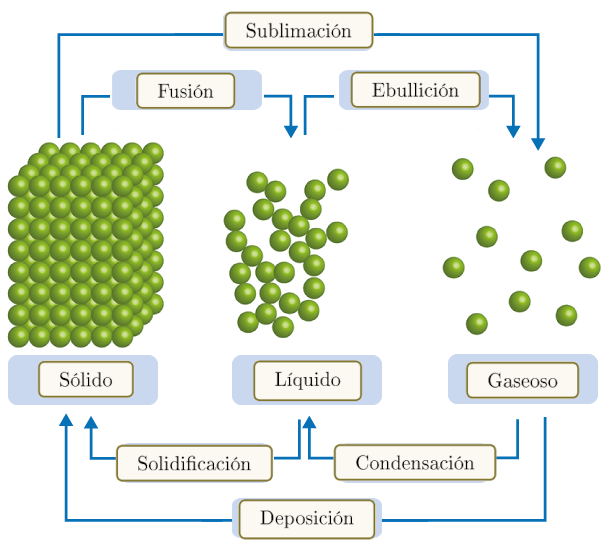
\includegraphics[width=\linewidth]{../images/SINFI_U2_AC47_IMG1_SOL.png}
			}\else{
				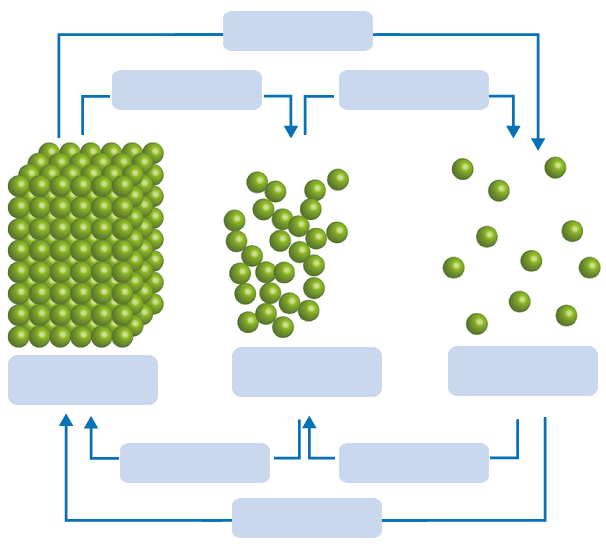
\includegraphics[width=\linewidth]{../images/SINFI_U2_AC47_IMG1.png}
			}\fi
		\end{minipage}
	}

	\questionboxed[5]{Elige la respuesta para cada pregunta, a partir de las imágenes de la figura \ref{fig:camiones3}.

		\begin{multicols}{2}
			\begin{figure}[H]
				\centering
				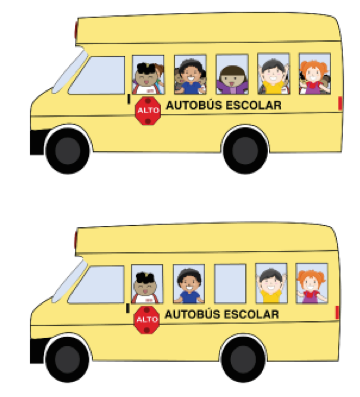
\includegraphics[width=0.5\linewidth]{camiones3.png}
				\caption{Dibujo de un autobus con muchos niños (arriba), y otro autobus con pocos niños.}
				\label{fig:camiones3}
			\end{figure}

			\begin{parts}
				\part  ¿Cuál podría aumentar más rápido su velocidad?

				\begin{checkboxes}
					\choice El autobús con más niños.
					\choice El autobús con menos niños.
					\choice Los dos autobuses aumentan su velocidad con la misma
					rapidez.
				\end{checkboxes}

				\part Si ambos autobuses se mueven a la misma velocidad, ¿a cuál de
				ellos le resultaría más difícil frenar?

				\begin{checkboxes}
					\choice Los dos autobuses requieren el mismo esfuerzo.
					\choice  El autobús con menos niños.
					\choice El autobús con más niños.
				\end{checkboxes}

				\part	Si la masa del segundo autobús es la mitad del primero
				y ambos conductores pisan el acelerador con la misma fuerza y mantienen
				el autobús en la misma dirección, ¿qué pasa con su aceleración?

				\begin{checkboxes}
					\choice Se mantiene igual.
					\choice Es el doble que la del primero.
					\choice Es la mitad de la del primero.
				\end{checkboxes}

				\part  Si el conductor del autobús baja a algunos niños,
				de tal manera que su masa sea sólo un cuarto de su masa inicial, cuando
				el conductor pisa el acelerador con la misma fuerza y mantiene el
				camión en la
				misma dirección, ¿qué pasa con su acelaración?

				\begin{checkboxes}
					\choice Aumenta cuatro veces.
					\choice Se mantiene igual.
					\choice Disminuye a la cuarta parte.
				\end{checkboxes}

				\part El conductor del autobús da vuelta hacia la derecha y los niños
				sienten una \emph{fuerza} que los empuja. ¿En qué dirección sienten los
				niños esta fuerza?

				\begin{checkboxes}
					\choice Los niños sienten que son empujados hacia abajo.
					\choice Los niños sienten que son empujados hacia la derecha del
					autobús.
					\choice Los niños sienten que son empujados hacia la izquierda del
					autobús.
				\end{checkboxes}
			\end{parts}
		\end{multicols}
	}


	\questionboxed[10]{Elige la respuesta para cada pregunta, a partir de las imágenes de la figura \ref{fig:camionesdecarga01}.

		\begin{multicols}{2}
			\begin{figure}[H]
				\centering
				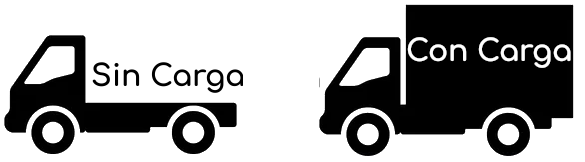
\includegraphics[width=0.8\linewidth]{../images/camionesdecarga01}
				\label{fig:camionesdecarga01}
				\caption{Representación de dos vehículos de carga.}
			\end{figure}

			\begin{parts}
				\part  ¿Cuál de ellos será más fácil poner en movimiento?

				\begin{oneparcheckboxes}
					\choice El camión sin carga.
					\choice El camión cargado. \\
					\choice Los dos camiones requieren el mismo esfuerzo.
				\end{oneparcheckboxes}

				\part  Si ambos camiones se movieran a la misma velocidad,
				¿a cuál de ellos le resultaría más fácil frenar?

				\begin{oneparcheckboxes}
					\choice El camión sin carga.
					\choice El camión cargado. \\
					\choice Los dos camiones requieren el mismo esfuerzo.
				\end{oneparcheckboxes}

				\part  ¿Cuál podría aumentar más rápido su velocidad?

				\begin{oneparcheckboxes}
					\choice El camión sin carga.
					\choice El camión cargado. \\
					\choice Los dos camiones aumentan su velocidad con la misma
					rapidez.
				\end{oneparcheckboxes}

				\part  ¿Cuál de los camiones podría tomar una curva con más
				facilidad si ambos se están moviendo a la misma velocidad?

				\begin{oneparcheckboxes}
					\choice El camión sin carga.
					\choice El camión cargado. \\
					\choice Los dos camiones requieren el mismo esfuerzo.
				\end{oneparcheckboxes}

				\part ¿Cuál de ellos será más difícil poner en movimiento?
				\begin{oneparcheckboxes}
					\choice El camión sin carga.
					\choice El camión cargado. \\
					\choice Los dos camiones requieren el mismo esfuerzo.
				\end{oneparcheckboxes}

				\part ¿Cuál podría aumentar más lento su velocidad?

				\begin{oneparcheckboxes}
					\choice El camión sin carga.
					\choice El camión cargado. \\
					\choice Los dos camiones aumentan su velocidad con la misma rapidez.
				\end{oneparcheckboxes}

				\part Si ambos camiones se movieran a la misma velocidad,
				¿a cuál de ellos le resultaría más difícil frenar?

				\begin{oneparcheckboxes}
					\choice El camión sin carga.
					\choice El camión cargado. \\
					\choice Los dos camiones requieren el mismo esfuerzo.
				\end{oneparcheckboxes}

				\part ¿Cuál de los camiones podría tomar una curva con más
				dificultad si ambos se están moviendo a la misma velocidad?

				\begin{oneparcheckboxes}
					\choice El camión sin carga.
					\choice El camión cargado. \\
					\choice Los dos camiones requieren el mismo esfuerzo.
				\end{oneparcheckboxes}

				\part Si se reduce la carga de arena de tal manera que la masa
				del camión sea la mitad de su masa inicial, mientras el conductor pisa el
				acelerador con la misma fuerza y mantiene el camión en la misma dirección,
				¿qué pasa con la acelaración del camión?

				\begin{oneparcheckboxes}
					\choice Aumenta al doble.
					\choice Disminuye a la mitad.\\
					\choice No cambia.
				\end{oneparcheckboxes}
				%\vspace{1cm}

				\part  Si el camión cargado va dejando gradualmente parte de su
				cargamento mientras el
				conductor pisa el acelerador con la misma fuerza y mantiene el camión
				en la misma dirección,
				¿qué pasa con su rapidez?

				\begin{oneparcheckboxes}
					\choice Aumenta.
					\choice Disminuye.
					\choice No cambia.
				\end{oneparcheckboxes}
			\end{parts}
		\end{multicols}
	}

	

\end{questions}
\end{document}